\documentclass[11pt]{article}
\usepackage{physics,slashed}




% NOTE: Add in the relevant information to the commands below; or, if you'll be using the same information frequently, add these commands at the top of paolo-pset.tex file. 
\newcommand{\name}{TA: Hossein Mohammadi}
\newcommand{\email}{hossein.mohammadi.00427@gmail.com}
\newcommand{\classnum}{Advanced Quantum Field Theory}
\newcommand{\subject}{Subject: Renormalized Perturbation Theory, IR Divergences, and Renormalization of QED}
\newcommand{\instructors}{Dr. Amin Faraji}
\newcommand{\assignment}{PSet 6}
\newcommand{\semester}{- Fall 1402}
\newcommand{\duedate}{dd/mm/yyyy}

% Copyright 2021 Paolo Adajar (padajar.com, paoloadajar@mit.edu)
% 
% Permission is hereby granted, free of charge, to any person obtaining a copy of this software and associated documentation files (the "Software"), to deal in the Software without restriction, including without limitation the rights to use, copy, modify, merge, publish, distribute, sublicense, and/or sell copies of the Software, and to permit persons to whom the Software is furnished to do so, subject to the following conditions:
%
% The above copyright notice and this permission notice shall be included in all copies or substantial portions of the Software.
% 
% THE SOFTWARE IS PROVIDED "AS IS", WITHOUT WARRANTY OF ANY KIND, EXPRESS OR IMPLIED, INCLUDING BUT NOT LIMITED TO THE WARRANTIES OF MERCHANTABILITY, FITNESS FOR A PARTICULAR PURPOSE AND NONINFRINGEMENT. IN NO EVENT SHALL THE AUTHORS OR COPYRIGHT HOLDERS BE LIABLE FOR ANY CLAIM, DAMAGES OR OTHER LIABILITY, WHETHER IN AN ACTION OF CONTRACT, TORT OR OTHERWISE, ARISING FROM, OUT OF OR IN CONNECTION WITH THE SOFTWARE OR THE USE OR OTHER DEALINGS IN THE SOFTWARE.

\usepackage{fullpage}
\usepackage{enumitem}
\usepackage{amsfonts, amssymb, amsmath,amsthm}
\usepackage{mathtools}
\usepackage[pdftex, pdfauthor={\name}, pdftitle={\classnum~\assignment}]{hyperref}
\usepackage[dvipsnames]{xcolor}
\usepackage{bbm}
\usepackage{graphicx}
\usepackage{mathrsfs}
\usepackage{pdfpages}
\usepackage{tabularx}
\usepackage{pdflscape}
\usepackage{makecell}
\usepackage{booktabs}
\usepackage{natbib}
\usepackage{caption}
\usepackage{subcaption}
\usepackage{physics}
\usepackage[many]{tcolorbox}
\usepackage{version}
\usepackage{ifthen}
\usepackage{cancel}
\usepackage{listings}
\usepackage{courier}

\usepackage{tikz}
\usepackage{istgame}
\usepackage{Float}

\hypersetup{
	colorlinks=true,
	linkcolor=blue,
	filecolor=magenta,
	urlcolor=blue,
}

\setlength{\parindent}{0mm}
\setlength{\parskip}{2mm}

\setlist[enumerate]{label=({\alph*})}
\setlist[enumerate, 2]{label=({\roman*})}

\allowdisplaybreaks[1]

\newcommand{\psetheader}{
	\ifthenelse{\isundefined{\collaborators}}{
		\begin{center}
			{\setlength{\parindent}{0cm} \setlength{\parskip}{0mm}
				
				\textbf{\classnum~\semester:~\assignment} \hfill \name
				
				
				\subject \hfill %\href{mailto:\email}{\tt \email}
				
				Instructor:~\instructors \hfill Due Date:~\duedate	
				
				\hrulefill}
		\end{center}
	}{
		\begin{center}
			{\setlength{\parindent}{0cm} \setlength{\parskip}{0mm}
				
				{\textbf{\classnum~\semester:~\assignment} \hfill \name\footnote{Collaborator(s): \collaborators}}
				
				\subject \hfill \href{mailto:\email}{\tt \email}
				
				Instructor(s):~\instructors \hfill Due Date:~\duedate	
				
				\hrulefill}
		\end{center}
	}
}

\renewcommand{\thepage}{\classnum~\assignment \hfill \arabic{page}}

\makeatletter
\def\points{\@ifnextchar[{\@with}{\@without}}
\def\@with[#1]#2{{\ifthenelse{\equal{#2}{1}}{{[1 point, #1]}}{{[#2 points, #1]}}}}
\def\@without#1{\ifthenelse{\equal{#1}{1}}{{[1 point]}}{{[#1 points]}}}
\makeatother

\newtheoremstyle{theorem-custom}%
{}{}%
{}{}%
{\itshape}{.}%
{ }%
{\thmname{#1}\thmnumber{ #2}\thmnote{ (#3)}}

\theoremstyle{theorem-custom}

\newtheorem{theorem}{Theorem}
\newtheorem{lemma}[theorem]{Lemma}
\newtheorem{example}[theorem]{Example}

\newenvironment{problem}[1]{\color{black} #1}{}

\newenvironment{solution}{%
	\leavevmode\begin{tcolorbox}[breakable, colback=green!5!white,colframe=green!75!black, enhanced jigsaw] \proof[\scshape Solution:] \setlength{\parskip}{2mm}%
	}{\renewcommand{\qedsymbol}{$\blacksquare$} \endproof \end{tcolorbox}}

\newenvironment{reflection}{\begin{tcolorbox}[breakable, colback=black!8!white,colframe=black!60!white, enhanced jigsaw, parbox = false]\textsc{Reflections:}}{\end{tcolorbox}}

\newcommand{\qedh}{\renewcommand{\qedsymbol}{$\blacksquare$}\qedhere}

\definecolor{mygreen}{rgb}{0,0.6,0}
\definecolor{mygray}{rgb}{0.5,0.5,0.5}
\definecolor{mymauve}{rgb}{0.58,0,0.82}

% from https://github.com/satejsoman/stata-lstlisting
% language definition
\lstdefinelanguage{Stata}{
	% System commands
	morekeywords=[1]{regress, reg, summarize, sum, display, di, generate, gen, bysort, use, import, delimited, predict, quietly, probit, margins, test},
	% Reserved words
	morekeywords=[2]{aggregate, array, boolean, break, byte, case, catch, class, colvector, complex, const, continue, default, delegate, delete, do, double, else, eltypedef, end, enum, explicit, export, external, float, for, friend, function, global, goto, if, inline, int, local, long, mata, matrix, namespace, new, numeric, NULL, operator, orgtypedef, pointer, polymorphic, pragma, private, protected, public, quad, real, return, rowvector, scalar, short, signed, static, strL, string, struct, super, switch, template, this, throw, transmorphic, try, typedef, typename, union, unsigned, using, vector, version, virtual, void, volatile, while,},
	% Keywords
	morekeywords=[3]{forvalues, foreach, set},
	% Date and time functions
	morekeywords=[4]{bofd, Cdhms, Chms, Clock, clock, Cmdyhms, Cofc, cofC, Cofd, cofd, daily, date, day, dhms, dofb, dofC, dofc, dofh, dofm, dofq, dofw, dofy, dow, doy, halfyear, halfyearly, hh, hhC, hms, hofd, hours, mdy, mdyhms, minutes, mm, mmC, mofd, month, monthly, msofhours, msofminutes, msofseconds, qofd, quarter, quarterly, seconds, ss, ssC, tC, tc, td, th, tm, tq, tw, week, weekly, wofd, year, yearly, yh, ym, yofd, yq, yw,},
	% Mathematical functions
	morekeywords=[5]{abs, ceil, cloglog, comb, digamma, exp, expm1, floor, int, invcloglog, invlogit, ln, ln1m, ln, ln1p, ln, lnfactorial, lngamma, log, log10, log1m, log1p, logit, max, min, mod, reldif, round, sign, sqrt, sum, trigamma, trunc,},
	% Matrix functions
	morekeywords=[6]{cholesky, coleqnumb, colnfreeparms, colnumb, colsof, corr, det, diag, diag0cnt, el, get, hadamard, I, inv, invsym, issymmetric, J, matmissing, matuniform, mreldif, nullmat, roweqnumb, rownfreeparms, rownumb, rowsof, sweep, trace, vec, vecdiag, },
	% Programming functions
	morekeywords=[7]{autocode, byteorder, c, _caller, chop, abs, clip, cond, e, fileexists, fileread, filereaderror, filewrite, float, fmtwidth, has_eprop, inlist, inrange, irecode, matrix, maxbyte, maxdouble, maxfloat, maxint, maxlong, mi, minbyte, mindouble, minfloat, minint, minlong, missing, r, recode, replay, return, s, scalar, smallestdouble,},
	% Random-number functions
	morekeywords=[8]{rbeta, rbinomial, rcauchy, rchi2, rexponential, rgamma, rhypergeometric, rigaussian, rlaplace, rlogistic, rnbinomial, rnormal, rpoisson, rt, runiform, runiformint, rweibull, rweibullph,},
	% Selecting time-span functions
	morekeywords=[9]{tin, twithin,},
	% Statistical functions
	morekeywords=[10]{betaden, binomial, binomialp, binomialtail, binormal, cauchy, cauchyden, cauchytail, chi2, chi2den, chi2tail, dgammapda, dgammapdada, dgammapdadx, dgammapdx, dgammapdxdx, dunnettprob, exponential, exponentialden, exponentialtail, F, Fden, Ftail, gammaden, gammap, gammaptail, hypergeometric, hypergeometricp, ibeta, ibetatail, igaussian, igaussianden, igaussiantail, invbinomial, invbinomialtail, invcauchy, invcauchytail, invchi2, invchi2tail, invdunnettprob, invexponential, invexponentialtail, invF, invFtail, invgammap, invgammaptail, invibeta, invibetatail, invigaussian, invigaussiantail, invlaplace, invlaplacetail, invlogistic, invlogistictail, invnbinomial, invnbinomialtail, invnchi2, invnF, invnFtail, invnibeta, invnormal, invnt, invnttail, invpoisson, invpoissontail, invt, invttail, invtukeyprob, invweibull, invweibullph, invweibullphtail, invweibulltail, laplace, laplaceden, laplacetail, lncauchyden, lnigammaden, lnigaussianden, lniwishartden, lnlaplaceden, lnmvnormalden, lnnormal, lnnormalden, lnwishartden, logistic, logisticden, logistictail, nbetaden, nbinomial, nbinomialp, nbinomialtail, nchi2, nchi2den, nchi2tail, nF, nFden, nFtail, nibeta, normal, normalden, npnchi2, npnF, npnt, nt, ntden, nttail, poisson, poissonp, poissontail, t, tden, ttail, tukeyprob, weibull, weibullden, weibullph, weibullphden, weibullphtail, weibulltail,},
	% String functions 
	morekeywords=[11]{abbrev, char, collatorlocale, collatorversion, indexnot, plural, plural, real, regexm, regexr, regexs, soundex, soundex_nara, strcat, strdup, string, strofreal, string, strofreal, stritrim, strlen, strlower, strltrim, strmatch, strofreal, strofreal, strpos, strproper, strreverse, strrpos, strrtrim, strtoname, strtrim, strupper, subinstr, subinword, substr, tobytes, uchar, udstrlen, udsubstr, uisdigit, uisletter, ustrcompare, ustrcompareex, ustrfix, ustrfrom, ustrinvalidcnt, ustrleft, ustrlen, ustrlower, ustrltrim, ustrnormalize, ustrpos, ustrregexm, ustrregexra, ustrregexrf, ustrregexs, ustrreverse, ustrright, ustrrpos, ustrrtrim, ustrsortkey, ustrsortkeyex, ustrtitle, ustrto, ustrtohex, ustrtoname, ustrtrim, ustrunescape, ustrupper, ustrword, ustrwordcount, usubinstr, usubstr, word, wordbreaklocale, worcount,},
	% Trig functions
	morekeywords=[12]{acos, acosh, asin, asinh, atan, atanh, cos, cosh, sin, sinh, tan, tanh,},
	morecomment=[l]{//},
	% morecomment=[l]{*},  // `*` maybe used as multiply operator. So use `//` as line comment.
	morecomment=[s]{/*}{*/},
	% The following is used by macros, like `lags'.
	morestring=[b]{`}{'},
	% morestring=[d]{'},
	morestring=[b]",
	morestring=[d]",
	% morestring=[d]{\\`},
	% morestring=[b]{'},
	sensitive=true,
}

\lstset{ 
	backgroundcolor=\color{white},   % choose the background color; you must add \usepackage{color} or \usepackage{xcolor}; should come as last argument
	basicstyle=\footnotesize\ttfamily,        % the size of the fonts that are used for the code
	breakatwhitespace=false,         % sets if automatic breaks should only happen at whitespace
	breaklines=true,                 % sets automatic line breaking
	captionpos=b,                    % sets the caption-position to bottom
	commentstyle=\color{mygreen},    % comment style
	deletekeywords={...},            % if you want to delete keywords from the given language
	escapeinside={\%*}{*)},          % if you want to add LaTeX within your code
	extendedchars=true,              % lets you use non-ASCII characters; for 8-bits encodings only, does not work with UTF-8
	firstnumber=0,                % start line enumeration with line 1000
	frame=single,	                   % adds a frame around the code
	keepspaces=true,                 % keeps spaces in text, useful for keeping indentation of code (possibly needs columns=flexible)
	keywordstyle=\color{blue},       % keyword style
	language=Octave,                 % the language of the code
	morekeywords={*,...},            % if you want to add more keywords to the set
	numbers=left,                    % where to put the line-numbers; possible values are (none, left, right)
	numbersep=5pt,                   % how far the line-numbers are from the code
	numberstyle=\tiny\color{mygray}, % the style that is used for the line-numbers
	rulecolor=\color{black},         % if not set, the frame-color may be changed on line-breaks within not-black text (e.g. comments (green here))
	showspaces=false,                % show spaces everywhere adding particular underscores; it overrides 'showstringspaces'
	showstringspaces=false,          % underline spaces within strings only
	showtabs=false,                  % show tabs within strings adding particular underscores
	stepnumber=2,                    % the step between two line-numbers. If it's 1, each line will be numbered
	stringstyle=\color{mymauve},     % string literal style
	tabsize=2,	                   % sets default tabsize to 2 spaces
%	title=\lstname,                   % show the filename of files included with \lstinputlisting; also try caption instead of title
	xleftmargin=0.25cm
}


% NOTE: To compile a version of this pset without problems, solutions, or reflections, uncomment the relevant line below.

%\excludeversion{problem}
%\excludeversion{solution}
%\excludeversion{reflection}

\begin{document}	
	
	% Use the \psetheader command at the beginning of a pset. 
	\psetheader
	
	\section*{Problem 1: Renormalization of Yukawa Theory}
	
	\begin{problem}
		We've talked about the renormalized propagator of fermions in Yukawa theory. This exercise aims to complete the renormalization of this theory in one loop level. Consider Yukawa theory with the following Lagrangian:
		\[
		\mathcal{L} = \frac12 (\partial_\mu \phi)^2 - \frac12 m^2\phi^2 +\bar{\psi} (i\slashed{\partial}-M)\psi -ig\bar{\psi} \gamma^5 \psi \phi
		\]
		
	\end{problem}
	\begin{enumerate}
		\item
		\begin{problem}{\points{-}}
			\textbf{Correction to the Scalar Two-point Function:}
			
			\begin{enumerate}
				\item 
			
			Compute the one-loop contribution to the fermion two-point function, the figure below\footnote{Recall that the solid line is a fermionic particle, and the dashed line is the scalar particle.}.
			
			\begin{figure}[H]
				\centering
				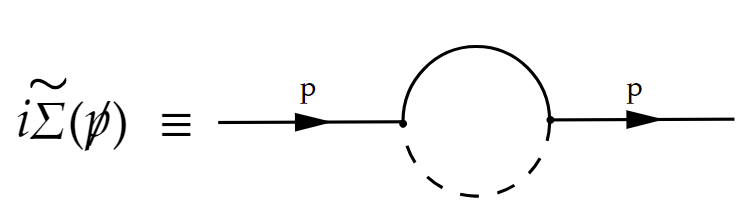
\includegraphics[width=0.45\linewidth]{img/1.png}
				\caption{Scalar propagator at one-loop level in Yukawa Theory.}
				\label{yukawa1}
			\end{figure}
			
		\item	Justify that the full two-point function up to $g^2$ order has the following contributions:
		\begin{equation*}
			i\Gamma(\slashed{p}) = \underbrace{i(\slashed{p}-M)}_{\text{Free part}} - \underbrace{i\tilde{\Sigma}(\slashed{p})}_{\text{Loop contribution}} + i \underbrace{(\delta_{Z_\psi}\slashed{p} - (\delta_M+\delta_{Z_\psi})M_R)}_{\text{Counterterms}}
		\end{equation*}
			\textbf{Hint:} Enter wavefunction and mass renormalization, $Z_\psi \text{ and } Z_M$, in the Lagrangian and exapnd around their tree level. Find their Feynman rule to reach the proposed form.
			\item 
			By requiring that
			\begin{equation}
				\begin{aligned}
					&\tilde{\Sigma}(\slashed{p} = 0) + \delta_M = 0
					\\&
					\frac{d}{d \slashed{p}} \tilde{\Sigma}(\slashed{p}) \Big|_{\slashed{p} = 0} = \delta_{Z_\psi}
				\end{aligned}
			\end{equation}
		which we will justify in the next problem, find the counterterms. Leave out the finite part of integrations and just write the exact form of the divergent part in the dimensional regularization.
		\end{enumerate}
	
	
	
	
	
	
			
		
		
		\end{problem}
	
		\item
		\begin{problem}{\points{-}}
		\textbf{Fermion-Fermion-Scalar Vertex Correction:}
		
		We pursue a similar path to renormalize the interaction vertex.
		 
		\begin{figure}[H]
			\centering
			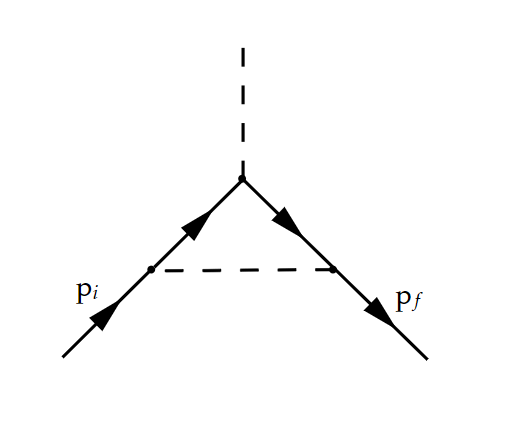
\includegraphics[width=0.3\linewidth]{img/2.png}
			\caption{The Loop contributing to the vertex correction in Yukawa Theory.}
			\label{yuk2}
		\end{figure}
\begin{enumerate}
	\item Write out its amplitude $V(p_f,p_i)$.
	\item Justify that the full amplitude of this three-point function up to $g^2$ order is:
	\[
	-i\Gamma (p_f,p_i) = \underbrace{g\gamma^5}_{\text{The usual interaction rule}} - \underbrace{iV(p_f,p_i)}_{\text{Loop correction}} +\underbrace{\delta_g \gamma^5}_{\textbf{Counterterm}}
	\]
	with entering vertex renormalization factor, $Z_g$, and expanding around tree level. ($Z_g = 1 + \delta_g$)
	\item Use the condition
	\[
	-i\Gamma(0,0) = g\gamma^5 -iV(0,0) + \delta_g \gamma^5 \equiv g_R \gamma^5
	\]
	\item By doing a similar procedure to the previous section of this problem, find the $\delta_g$ counterterm.

\end{enumerate}
	
		\end{problem}

\end{enumerate}

\newpage
	\section*{Problem 2: The Anomalous Magnetic Moment }
 
%This is a text $\vcenter{\hbox{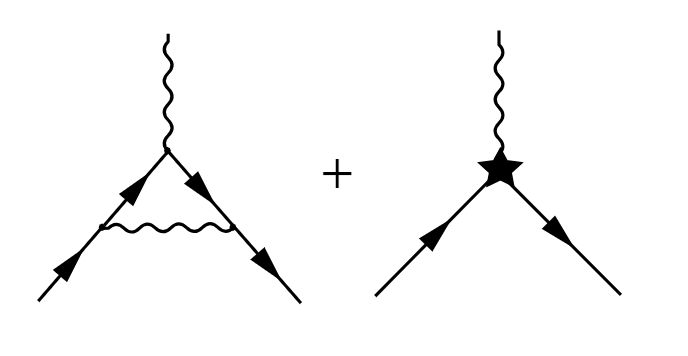
\includegraphics[height= 4.5 em]{img/inline.png}}}$ with a great alignemnt.

\begin{problem}
	In this problem, we carefully work out diagram \ref{ammom} and find the $g$-factor, which quantifies the strength of electron spin coupling to an external magnetic field.
	\begin{figure}[H]
		\centering
		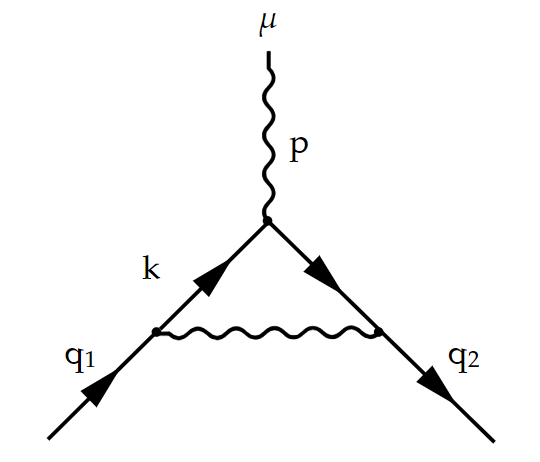
\includegraphics[width=0.3\linewidth]{img/3.png}
		\caption{Vacuum Polarization diagram in QED.}
		\label{ammom}
	\end{figure}
	\end{problem}

\begin{enumerate}
	\item
	\begin{problem}{\points{-}}
		\textbf{The amplitude:}
		
		Write down the amplitude of this diagram. (You have to write all fermionic propagators with slashed quantities in the numerator: $\frac{i}{\slashed{p}-m} \to i\frac{\slashed{p}+m}{p^2-m^2}$ )
	\end{problem}
\item
\begin{problem}{\points{-}}
	\textbf{Squaring the denominator:}
	
	Using 
	\[
	\frac{1}{ABC} = 2\int_0^1 dxdydz \delta(x+y+z-1) \frac{1}{(Ax+By+Cz)^3}
	\],
	write the denominator of this amplitude in a squared form. You have to end up 
	\[
	Ax+By+Cz = (k^\mu + yp^\mu -zq_1^\mu)^2 - \Delta +i\varepsilon
	\]
	with $\Delta = -xyp^2 + (1-z)^2m^2$.
	
\end{problem}
\item
\begin{problem}{\points{-}}
	\textbf{Simplify the numerator:}
	
	There is a quantity in the numerator, which is $\tr$ of spinorial objects, that gets complicated when we do a shift of variables. So it is a good idea to simplify it before shifting.
	
	Use arguments like vanishing of integrals, on-shell fermionic in-states, etc., to drop some terms and reach the following form for the numerator.
	\[
	-2 \bar{u}(q_2) \big(
	\slashed{k} \gamma^\mu \slashed{p} + \slashed{k} \gamma^\mu \slashed{k} + m^2 \gamma^\mu - 2m(2k+p)^\mu
	\big)
	u(q_1)
	\]
	
\end{problem}
\item
\begin{problem}{\points{-}}
	\textbf{Shift of variables:}
	
	As its form suggests, do $k^\mu \to k^\mu -yp^\mu +zq_1^\mu$. It is rather obvious that the Jacobian of this transformation equals to the unit.
	
\end{problem}
\item
\begin{problem}{\points{-}}
	\textbf{Simplify the numerator again:}
	
		Now there's a little technical and long calculation. Show that after applying the above transformation to the numerators we have to end up with
		\begin{equation}
			\begin{aligned}
			-\frac12 N^\mu = &\Big[
			-\frac12 k^2 + (1-x)(1-y)p^2 + (1-4z+z^2)m^2
			\Big] \bar{u}(q_2)\gamma^\mu u(q_1)
			\\&
			+imz(1-z) p_\nu \bar{u}(q_2)\sigma^{\mu\nu}u(q_1) 
			\\&
			+ m(z-2)(x-y)p^\mu \bar{u}(q_2)u(q_1)
		\end{aligned}
	\label{boringeq}
		\end{equation}
	
	There are several identities that you should utilize.
	\begin{itemize}
		\item $k^\mu k^\nu = \frac{1}{d} \eta^{\mu\nu} k^2$ under integration.
		\item Gordon Identity:
		\[
		\bar{u}(q_2)(q_1+q_2)^\mu u(q_1) = 2m\bar{u}(q_2)\gamma^\mu u(q_1) + i \bar{u}(q_2) \sigma^{\mu\nu} (q_1-q_2)_\nu u(q_1) 
		\]
		\item $x+y+z=1$, as it's also obvious from Dirac's delta function.
		\item $\tr(\gamma^\mu\gamma^\nu) = 4\eta^{\mu\nu}$.
		\item $\tr (\gamma^\alpha\gamma^\mu\gamma^\beta\gamma^\nu) = 4\big(
		\eta^{\alpha\mu}\eta^{\beta\nu}-\eta^{\alpha\beta}\eta^{\mu\nu}+\eta^{\alpha\nu}\eta^{\beta\mu}
		\big)$
	\end{itemize}
		
\end{problem}

\item
\begin{problem}{\points{-}}
	\textbf{$g$-factor:}
	
	As we have discussed, the $g$-factor only comes from the $\sigma^{\mu\nu}$ part of the amplitude. Even though there are divergences arising from other terms in \ref{boringeq}, we neglect them for the moment.
	
	So we have concluded that the part of amplitude that contributes to the $g$-factor is:
	\begin{equation}
	i\tilde{\mathcal{M}}^\mu_2 = p_\nu \bar{u}(q_2) \sigma^{\mu\nu} u(q_1)\Big(
	4ie^3m \int_0^1 dxdydz \delta(x+y+z-1) \times \int \frac{d^4k}{(2\pi)^4} \frac{z(1-z)}{(k^2-\Delta+i\varepsilon)^3}
	\Big)
	\label{gfac}
	\end{equation}
	Recall that the $g$-factor is choosen to be $\frac{4m}{e}$ times the coefficient of  $p_\nu \bar{u}(q_2) \sigma^{\mu\nu} u(q_1)$ in the amplitude, evaluated at $p^2=0$. Therefore, you can find the $g-$ factor in the loop level by doing a simple triple integration. Show that 
	\[
	g = 2 + \frac{\alpha}{\pi} = 2.00232
	\]
\end{problem}
\textbf{Caution:} All your calculations should be complete and detailed. In any stage, you can consult Schwartz's book, chapter 17, to guide you.

\end{enumerate}

\newpage
	\section*{Problem 3: Electron Self-Energy and Subtraction Schemes}
	Another two-point function in QED is
	\begin{figure}[H]
		\centering
		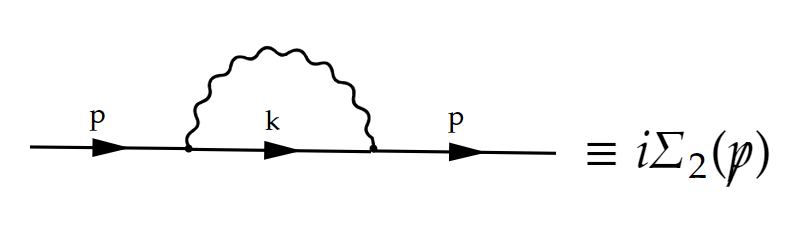
\includegraphics[width=0.5\linewidth]{img/4.png}
		\caption{QED fermionic self-energy graph.}
		\label{qedself}
	\end{figure}
	which needs two counterterms to be renormalized, as we will figure out.
	
\begin{enumerate}
	\item
	\begin{problem}{\points{-}}
		\textbf{The Regularized Amplitude:} 
		
		Work out this diagram in the dimensional regularization, and find
		\[
		\Sigma_2(\slashed{p}) = -\frac{\alpha}{2\pi} \int_0^1 dx (2m-x\slashed{p}) \Big[
		\frac{2}{\varepsilon} + \ln(\frac{4\pi e^{-\gamma_E}\mu^2}{(1-x)(m^2-p^2x)})
		\Big].
		\]
		Hence, the divergent part reads:
		\[
		\Sigma_2(\slashed{p}) = \frac{\alpha}{\pi} \big(
		\frac{\slashed{p} - 4m}{2\varepsilon} + \text{finite}
		\big) 	
	\]
	\end{problem}

	\item
	\begin{problem}{\points{-}}
		\textbf{Two counterterms are required:} 
		
		Argue why we can not eliminate these divergences by only one counterterm for mass, or $\delta_m$?
		What quantity should also be manipulated to eliminate the other divergent part, proportinal to $\slashed{p}$?
	\end{problem}


\item
\begin{problem}{\points{-}}
	\textbf{Renormalized Propagator:} 
	 
	 After renormalizing $\psi_0$  and $m_0$, the renormalized fermionic propagator is:
	 \[
	 iG^R(\slashed{p}) = \frac{1}{Z_2}\frac{i}{\slashed{p}-m_0}+ \text{loops} = (\frac{1}{1+\delta_2})
	 (\frac{i}{\slashed{p} -m_R -\delta_m m_R})+ \text{loops}
	 \]
	
	Expand this propagator to find such form,
	\[
	\frac{i}{\slashed{p}-m_R} + \frac{i}{\slashed{p}-m_R}\Big[
	i(\delta_2\slashed{p} - (\delta_2+\delta_m) m_R)
	\Big]\frac{i}{\slashed{p}-m_R} + \text{loops}
	\]
	Now add the loop contribution and determine $\delta_2$ and $\delta_m$ such that divergences cancel. (Choose the dimensional regularization and neglect the finite part of the regularized amplitude ($MS-$scheme))
\end{problem}


\item
\begin{problem}{\points{-}}
	\textbf{Subtraction schemes:} 
	
	I have defined the on-shell subtraction scheme in the last session. Let us have an example to see how it works in practice. As you know, in O.S., the renormalized mass $m_R$ is set equal to pole mass $m_P$.
	
	 By definitions of the pole mass, which is the pole of the dressed propagator with residue $i$, the O.S. conditions are the following\footnote{Of course, to order $e_R^2$ in perturbation theory. The definition of pole mass is not perturbative, but our calculations are!}
	\begin{equation}
		\begin{aligned}
			&\delta_2 = - \frac{d}{d\slashed{p}} \Sigma_2(\slashed{p})\Big|_{\slashed{p} = m_P}
			\\&
			\delta_m m_P = \Sigma_2(m_P)
		\end{aligned}
	\end{equation}
Utilizing the second condition to find finite part of the $\Sigma_2(\slashed{p})$ in O.S. scheme.(Use Pauli-Villars regularization, refer to 18.11 Schwartz.)

The final result is:
\[
\Sigma_2(m_P) = -\frac{\alpha}{2\pi} m_P \big(
\frac32 \ln(\frac{\Lambda^2}{m_P^2}) + \frac34
\big)
\]
\end{problem}


\textbf{Aside:} Using the first condition has subtleties. In theories with massless vector particles, it often leads to divergent integrals. The way to regularize these integrals is to consider that the photon is massive, $m_\gamma\neq 0$. We are not going into the details of such a procedure, but I will describe it briefly in this problem set.

\textbf{Aside:} $M.S.$ scheme is a very convenient since we eliminate all the finite parts in the loop contributions. However, the problem of relating mass ($m_R$) in different schemes leads to a powerful constraint in particle physics, which using $M.S.$ in particle physics is very inconvenient! 
\end{enumerate}
\newpage
	\section*{Interlude: Renormalized Perturbation Theory}
		Renormalized perturbation theory is a systematic approach to tame all the infinities that areised while dealing with loops.
		
		The idea is to consider a renormalization, $Z_\#$, for all the parameters and fields in the theory. Then expand them around their classical value, $Z_\# = 1+ \delta_\#$. Then, match $\delta_\#$ in any order of perturbation theory with the loop amplitudes' divergences.
		
		For QED, consider the following renormalization factor:
		\begin{equation}
			\begin{aligned}
				&m_0 = Z_mm_R \\&
				e_0 = Z_e e_R \\&
				\psi^0 = \sqrt{Z_2} \psi^R \\&
				A_\mu^0 = \sqrt{Z_3} A_\mu^R
			\end{aligned}
		\label{renorz}
		\end{equation}

As you know, bare parameters are considered to be infinite, so the Z-coefficient on the right-hand side of \ref{renorz} are infinite, and renormalized quantities are designated to be finite.

By substitution, the QED Lagrangian would become:
\[
\mathcal{L} = -\frac14 Z_3 (\partial_\mu A_\nu^R -\partial_\nu A_\mu^R )^2 + iZ_2 \bar{\psi}_R \slashed{\partial} \psi_R - Z_2Z_m m_R  \bar{\psi}_R  \psi_R - e_R Z_e Z_2 \sqrt{Z_3}  \bar{\psi}_R \slashed{A} \psi_R
\]
Conventionally, $Z_1 \equiv Z_e Z_2 \sqrt{Z_3}$.

Next we expand these factors around the tree level.

\begin{equation*}
	\begin{aligned}
		&Z_1 = 1+\delta_1 \\&
		Z_2 = 1+\delta_2 \\&
		Z_3 = 1+\delta_3 \\&
		Z_m = 1+\delta_m
	\end{aligned}
\end{equation*}
where counterterms are functions of $e_R$, that is because we want the counterterms to cancel loop divergences in any order of perturbation theory.

Plugging them into Lagrangian and collecting similar terms would lead to:
\begin{equation*}
	\begin{aligned}
		\mathcal{L} &= -\frac14 {F_{\mu\nu}^R}^2+ i\bar{\psi}^R \slashed{\partial}\psi^R - m_R \bar{\psi}^R \psi^R -e_R \bar{\psi}^R \slashed{A^R}\psi^R
		\\& 
		-\frac14 \delta_3{F_{\mu\nu}^R}^2+ i\delta_2\bar{\psi}^R \slashed{\partial}\psi^R -(\delta_m+\delta_2) m_R \bar{\psi}^R \psi^R -e_R \delta_1\bar{\psi}^R \slashed{A^R}\psi^R
	\end{aligned}
\end{equation*}

In renormalized perturbation theory, counterterms appear as interactions and used in Feynman diagrams calculations to render the amplitudes finite, order by order. You can see their Feynman rule in momentum space in figure \ref{ctfeynrul}

\begin{figure}[H]
	\centering
	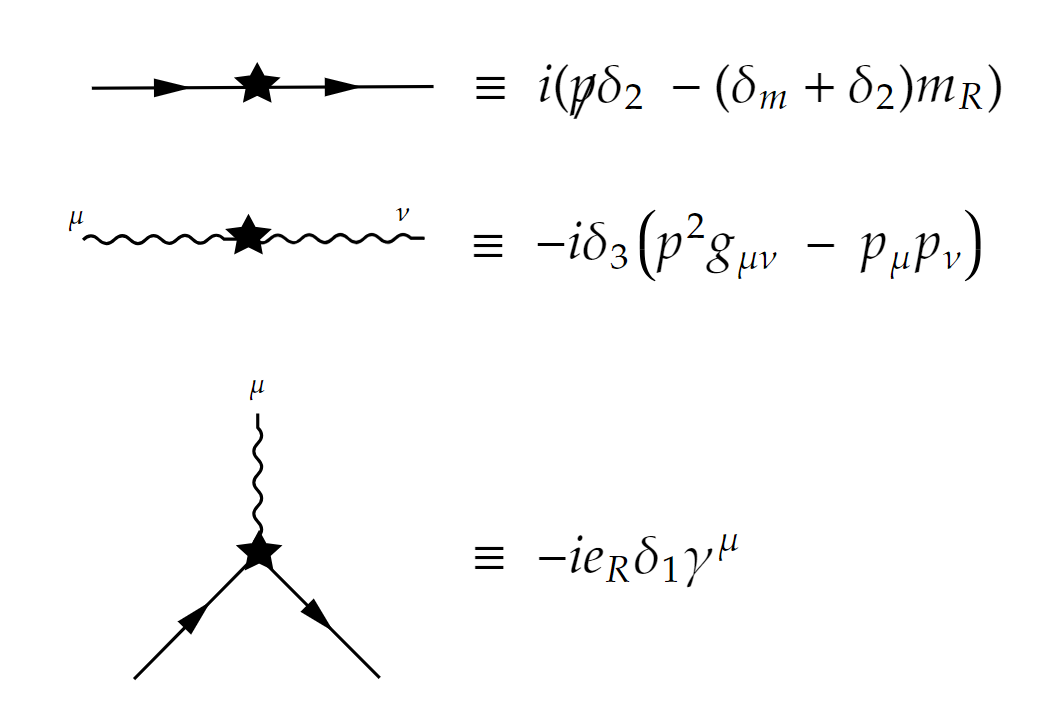
\includegraphics[width=0.65\linewidth]{img/5.png}
	\caption{Feynman rules for counterterm contributions in QED Lagrangian.}
	\label{ctfeynrul}
\end{figure}
Now, it is possible to justify perturbation theory since $e_R<1$.
\begin{enumerate}
		\item
	\begin{problem}{\points{-}}
		\textbf{Fermionic two-point function in renormalized perturbation theory:} 
		
		Draw three diagrams contributing to the fermionic propagator.One is at the tree level, and the other two are its loop correction and assicuated counterterms. Substitute their amplitude from problem 3 and compare your result with Problem 3 (c).
		
		\textbf{Aside:} By correcting this vertex, you will be able to find $\delta_m$ and $\delta_2$ counterterms in $e^2_R$ order. We have mentioned that finding them requires IR regularization, which you are invited to do for yourself. At the end we would have:
		\begin{equation}
			\delta_2 = \frac{e^2_R}{8\pi^2} \Big(
				-\frac{1}{\varepsilon} -\frac12 \ln(\frac{\tilde{\mu}^2}{m^2_R}) - \frac52 - \ln(\frac{m^2_\gamma}{m^2_R})
				\Big)
			\label{del2}.
		\end{equation}
	with $m_\gamma$ as the mass of photons, added to regularize the IR-divergence.
	\end{problem}
	
			\item
	\begin{problem}{\points{-}}
		\textbf{Photon propagator:}
		
		Add three contributions of tree-level, loop amplitude and counter terms for photon propagator.
		You saw that $\vcenter{\hbox{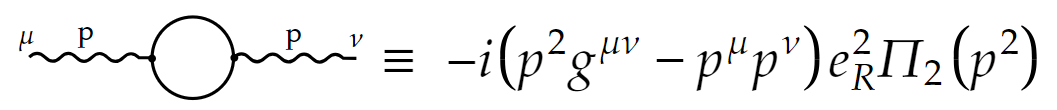
\includegraphics[height= 2.5 em]{img/6.png}}}$ with
		\[
		\Pi_2(p^2) = \frac{8}{(4\pi)^{\frac{d}{2}}} \Gamma(2-\frac{d}{2}) \mu^{4-d} \int_0^1 dx 
		\;x(1-x) \Big[
		\frac{1}{m^2_R - p^2x(1-x)}
		\Big]^{2-\frac{d}{2}}
		\]  
		Show that your renormalized propagator still satisfies Ward identity.
		
		\textbf{Aside:} In O.S. scheme, renormalization condition would be $\Pi(p^2=0) = \Pi(0) = 0$, with
		\begin{figure}[H]
			\centering
			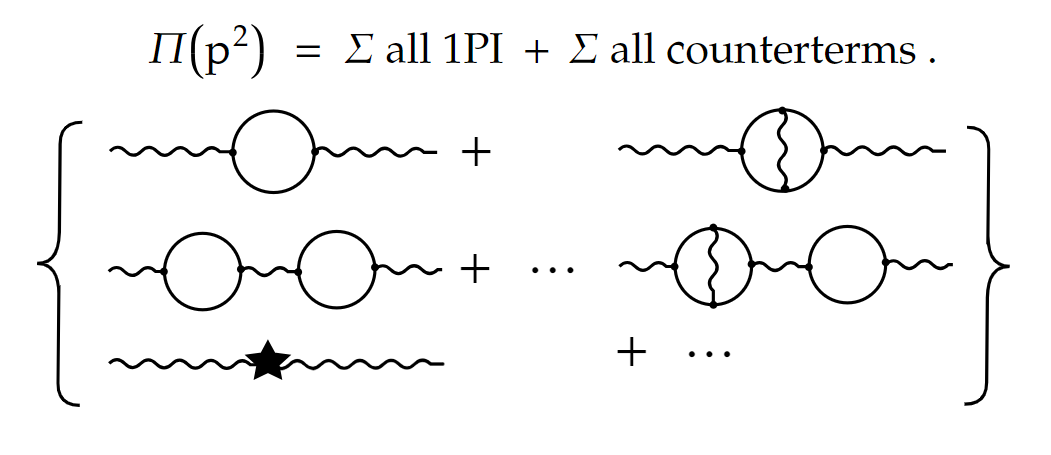
\includegraphics[width=0.65\linewidth]{img/7.png}
			\caption{Definition of the $\Pi(p^2)$, which is the non-tensorial part of the dressed propagator. }
			\label{Pitoallorders}
		\end{figure}
		The O.S. condition on $e^2_R$ order gives $\delta_3$,
		\[
		\delta_3 = -\frac{e^2_R}{6\pi^2}\frac{1}{\varepsilon} - \frac{e^2_R}{12\pi^2}\ln(\frac{\tilde{\mu}^2}{m^2_R})
		\]
		\end{problem}
			\item
	\begin{problem}{\points{-}}
		\textbf{Interaction vertex correction:}
		
		We have worked out the most general form of the amplitude of the interaction vertex\footnote{We have imposed Lorentz covariance and Ward identity constraints. Also, we supposed that incoming and outgoing fermions are on-shell. }:
		\begin{figure}[H]
			\centering
			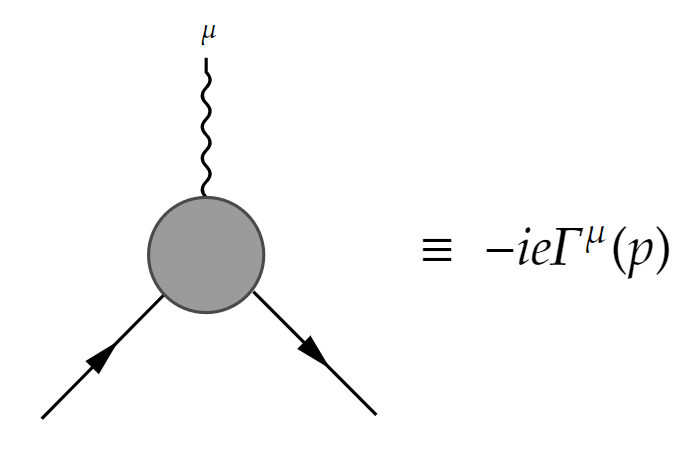
\includegraphics[width=0.4\linewidth]{img/8.png}
			\caption{The most general Feynman rule for QED vertex. 
					With
	$
		\Gamma^\mu (p) = F_1(p^2) \gamma^\mu+  \frac{i\sigma^{\mu\nu}}{2m_e} p_\nu F_2(p^2).
	$	
		}
			\label{blackboxver}
		\end{figure} 
	In the order $e^2_R$, $\vcenter{\hbox{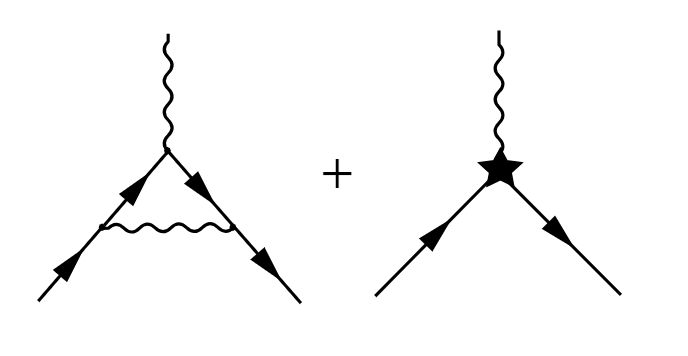
\includegraphics[height= 4.5 em]{img/inline.png}}}$ would add and we find the associated counterterm, $\delta_1$.
	
	Notice that we had not worked out this counterterm in problem 1, we just extracted the $\sigma^{\mu\nu}$ part to find the anomalous magnetic moment of the electron. This contribution is even harsher to compute. Fortunately, we do not need to calculate it since there is a strong condition between $Z_1$ and $Z_2$ in QED, namely $Z_1 = Z_2$. This implies that $\delta_1 = \delta_2$ in any order of perturabtion theory. 
	So by using \eqref{del2},
	\[
	\delta_1 = \delta_2 = \frac{e^2_R}{8\pi^2} \Big(
	-\frac{1}{\varepsilon} -\frac12 \ln(\frac{\tilde{\mu}^2}{m^2_R}) - \frac52 - \ln(\frac{m^2_\gamma}{m^2_R})
	\Big)
	\]
		
		\end{problem}
	
	
			\item
	\begin{problem}{\points{-}}
		\textbf{$\mathbf{Z_1 = Z_2}$ and its implications:}
		
		Read 19.5 Schwartz carefully and briefly discuss both the origin and the physical implication of this equality. Reflect how this is generalized in QCD. 
		
	\end{problem}
	
	\textbf{Aside:}
	We have worked out the following renormalization condition in one loop level
	\begin{equation*}
		\begin{aligned}
			&\Sigma(m_P) = 0 \\ &
			{\Sigma}^{'} (m_P) = 0 \\ &
			\Pi(0)=0 \\ &
			\Gamma^\mu(0)  = \gamma^\mu
		\end{aligned}
	\end{equation*}
	These conditions define countertems in all orders in QED and render all loops finite. The fact that we only need four counterterms to eliminate all loop divergences is QED's renormalizability. 
	\end{enumerate}
\newpage
\section*{Finally: Infrared divergences}

\begin{problem}
	I was going to cover this topic completely, but since you are already progressed at an astonishing pace, I would rather mention a few facts about IR divergences.
	
	As an instance, the $e^+e^- \to e^+e^-$ process (Bhabha scattering) has no finite amplitude after UV regularization in $e^4_R$ order; the divergence is due to integration on small momentum regions. The contributing diagrams up to $e^4_R$ are:
	\begin{figure}[H]
		\centering
		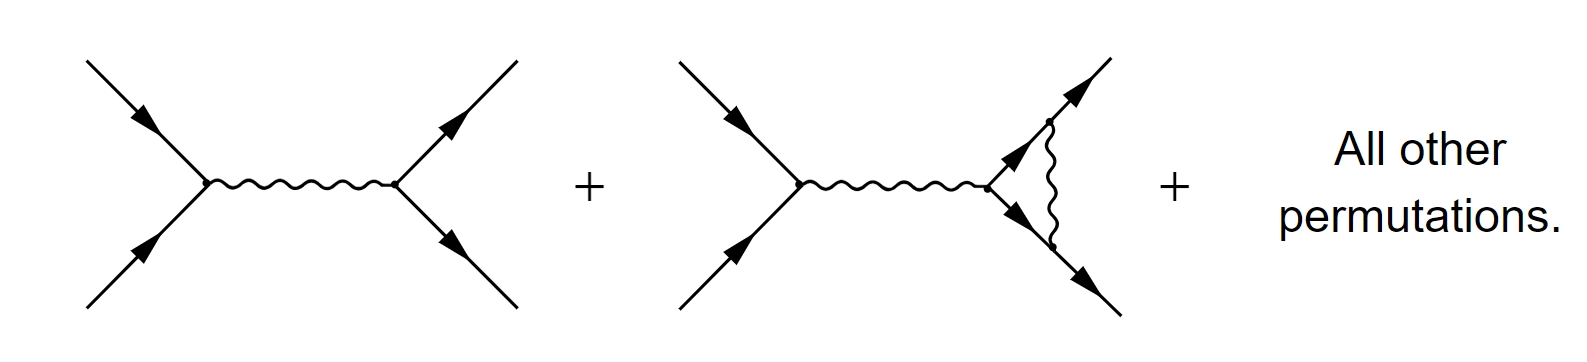
\includegraphics[width=0.95\linewidth]{img/9.png}
		\caption{Feynman diagrams contributing to Bhabha scattering.}
		\label{irdiv1}
	\end{figure}
	By considering a small mass for photon, $m_\gamma$, IR divergence could be tamed.
	\[
	\sigma_V = \frac{e^2_R}{8\pi^2} \sigma_0 \Bigl\{-\ln^2(\frac{m_\gamma^2}{Q^2}) -3\ln (\frac{m^2_\gamma}{Q^2}) -\frac72 + \frac{\pi^2}{3}\Bigr\}
	\]
	With $Q^2$, the "CM"-energy and $\sigma_0 = \frac{e^4_R}{12\pi Q^2}$ the tree level scattering cross section. Notice that we "MUST" compute the cross section, not the amplitude, to deal with IR infinities correctly.
	
	The double logarithm $\ln^2(\#)$ could not be remedied by comparing cross sections at different energy scales $Q_1$, $Q_2$.
	\[
	\sigma_V(Q_1^2)-\sigma_V(Q_2^2) =  \frac{e^2_R}{8\pi^2} \sigma_0 \Bigl\{-\ln^2(\frac{m_\gamma^2}{Q_1^2}) + \ln^2(\frac{m_\gamma^2}{Q_2^2}) -3\ln (\frac{Q_2^2}{Q_1^2})\Bigr\}
	\]
	The remedy comes from "Real Emission Graphs" (REG)\footnote{They are the same order in perturbation theory as the cross section of diagrams \ref{irdiv1}, but has more final states of the massless particle.
	
You might ask if these graphs are in order $e^3_R$, but the figure \ref{irdiv1} diagrams are $e^2_R$ and $e^4_R$, respectively. The clarification is the below figure 
\begin{figure}[H]
	\centering
	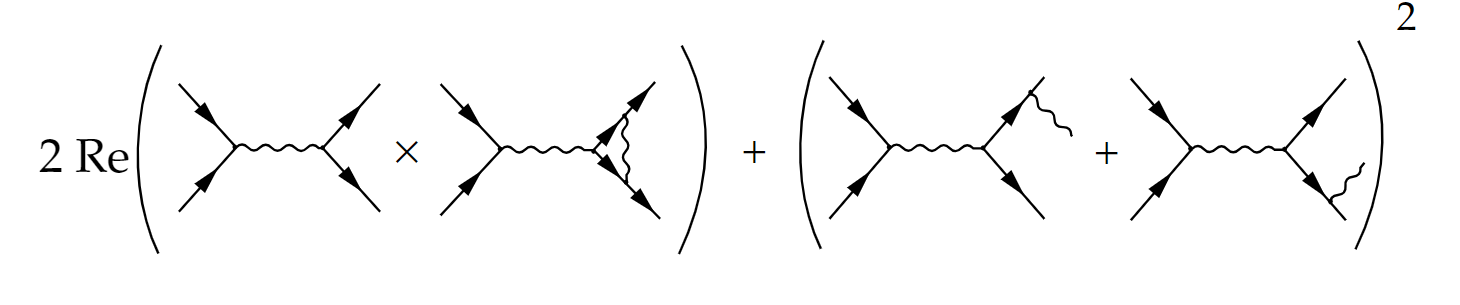
\includegraphics[width=0.85\linewidth]{img/11.png}
	\caption{Diagrams that add up to cancel IR infinities, only after working cross section, not amplitude.}
	\label{clarif}
\end{figure}
All the calculations are in order $e^6_R$. An even stronger statement is that you can take different charges for two fermionic vertices, namely $Q_e$ and $Q_\mu$ (showing the $e^+e^- \to \mu^+ \mu^-$ process) then all the diagrams in the $Q^3_e Q^3_\mu$ add up to cancel IR divergences.
}

\begin{figure}[H]
	\centering
	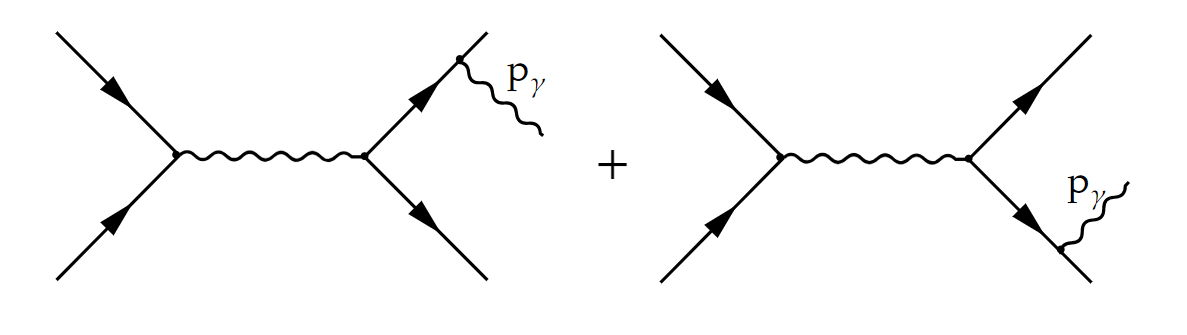
\includegraphics[width=0.75\linewidth]{img/10.png}
	\caption{Diagrams that add up to cancel IR infinities, only after working cross section, not amplitude.}
	\label{irdiv2}
\end{figure}
After working out its cross section, you will find:
\[
\sigma_R = \frac{e^2_R}{8\pi^2} \sigma_0 \Bigl\{+\ln^2(\frac{m_\gamma^2}{Q^2}) +3\ln (\frac{m^2_\gamma}{Q^2}) +5 - \frac{\pi^2}{3}\Bigr\}
\]
Fortunately, both $\ln^2(\#)$ and $\ln(\#)$ cancel, and we have 
\[
\sigma_{tot} = \sigma_0 \big(
1+ \frac{3e^2_R}{16\pi^2}
\big)
\].

The fact that one can not get rid of IR infinities unless adding REGs has a significant physical consequence. The final photon states in REGs are inevitable in experiments. It does not vanish when the resolution of the detectors is increased!

These graphs' calculations are boring, and at some stages, Mathematica is required. Weinberg elaborates this explanation about IR infinities more, I would suggest everyone read the final conclusions of Weinberg if they are engrossed.
\end{problem}










\end{document}